\documentclass[12pt,fleqn]{article}\usepackage{../common}
\begin{document}
Ders 29

Nihayet en son ayristirma (decomposition) konusuna geldik, bu teknik Tekil
Deger Ayristirma (Singular Value Decomposition -SVD-)
teknigidir. Ayristirma su halde olacak

\[ A = U \Sigma V^T \]

Sag tarafta ayrisma sonrasi bir ortogonal matris, bir kosegen (diagonal)
matris, ve tekrar bir ortogonal matris olacak. Yani bildigimiz, sevdigimiz
matris formlari ayrisma sonrasi parcalar olarak elimize gececekler. Ilginc
olan iki tane ortogonal matris elde etmemiz. Ayrica $A$ her turden, her
boyuttan bir matris olabilir (illa karesel olmasi gerekmez mesela).

SVD bu dersin pek cok kavramini da bir araya getirir. Mesela simetrik
pozitif kesin matrisler. Hatirlarsak bu matrisler simetrik oldugu icin
ozvektorleri ortogonal idi. Yani normalde su haldeki bir ayrisma

\[ A = S \Lambda S ^{-1}   \]

Su halde gorulebiliyordu

\[ A = Q \Lambda Q ^{T}   \]

Yani $S$, ortogonal vektorlu $Q$ oluyordu, pozitif kesinlik sayesinde de
normal bir $\Lambda$, icinde sadece pozitif degerler tasiyan bir  $\Lambda$
oluyordu. 

Ozetle, eger $A$ simetrik pozitif kesin ise onun SVD'si $Q \Lambda Q ^{T}$
olacaktir. Bu durumda tek $Q$ matrisi yeterli, diger durumlarda $U,V$ gibi
iki farkli matris lazim. Ayrica sunu da vurgulayalim: SVD icin ortogonallik
aradigimiz onemli bir sart, ``ortogonal carpi kosegen carpi ortogonal''
seklinde bir form istiyorum ozellikle. 

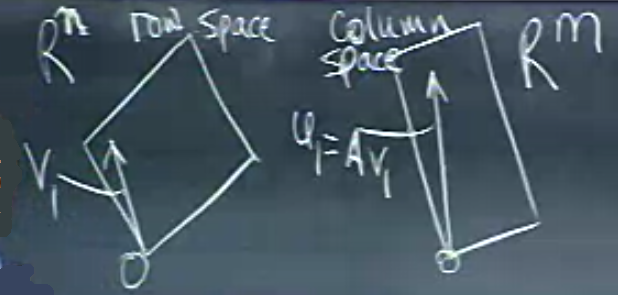
\includegraphics[height=4cm]{29_1.png}

SVD'den bekledigimiz islemi yukaridaki resim uzerinden anlamaya
calisalim. Soldaki duzlem satir uzayi (row space), sagdaki kolon uzayi
(column space). Bir matrisi temsil eden satirlar ve kolonlar bu uzaylarin
icinde. Simdi eger $U \Sigma V^T$ formunu dusunursek, oyle bir kosegen
matris ariyorum ki satir uzayindaki ortogonal bazi (basis) uzayindaki bir
ortogonal baza transform etmeli. Bu hakikaten ozel bir matris olmali.

Soru: satir uzayinin ortogonal bazi var midir? Tabii ki vardir,
Gram-Schmidt tekniginde gorduk, herhangi bir bazin ortogonal bazini
alabiliriz. Ortogonal baz hesabi ozgun degildir, ayni bazdan pek cok
ortogonal baz cikartilabilir, ve satir uzayindaki ``herhangi'' bir
ortogonal bazi alip kolon uzayina transform edersem onun illa ortogonal
kalacagi garanti degildir. Yani transform edildikten sonra da ortogonal
kalacak ozel bir ortogonal baz ariyorum. Yapmaya calistigim carpim her
vektoru gosterecek sekilde nasildir?

\[ 
A \left[\begin{array}{rrrr}
&&& \\
v_1 & v_2& ... & v_r \\
&&& 
\end{array}\right] = 
\left[\begin{array}{rrrr}
&&& \\
u_1 & u_2& ... & u_r \\
&&& 
\end{array}\right] 
\left[\begin{array}{rrrr}
\sigma_1 &&& \\
 & \sigma_2&  & \\
&& \ddots & \\
&&& \sigma_r
\end{array}\right] 
 \]

Yani $Av_1$ carpimi bana $u_1 \sigma_1$'i vermeli. Matris olarak yukaridaki 

\[ AV = U\Sigma \]

Hatta ortogonallikten daha ileride ortonormalligi hesaplamak daha da iyi. 

Ornek 

\[ 
A = 
\left[\begin{array}{rr}
4 & 4 \\ -3 & 3
\end{array}\right]
 \]

$A$ tersine cevirilebilir (invertible) o zaman kertesi (rank)
2. Aradiklarim 

\[ v_1,v_2 \  \mathbb{R}^2 \textit{ satir uzayinda }  \]

\[ u_1,u_2 \  \mathbb{R}^2 \textit{ kolon uzayinda }  \]

\[ \sigma_1 > 0, \sigma_2 > 0 \]

Sifir uzayi (nullspace) burada problem degil. Zorluklar neler? Matris
simetrik olmayabilir, o zaman ozvektorleri kullanamam, cunku onlar
ortogonal degildir.






















\end{document}
